%!TEX program = xelatex
%!TEX root = ./thesis.tex

\section{Hierarchical reinforcement learning methods for multi-modality and sparse environments}
This section will discuss the experiments on the proposed hierarchical reinforcement learning models.

In our experiment settings, we choose the set $\{move0, move1, \dots, move7 \}$ as source tasks. We select "dynamicg4" as a representative target task for multi-modality environments and "reachcont" as a representative target task for multi-modality sparse environments.

The problem of hierarchical reinforcement learning is divided into two parts: learning robust actuator policies and learning the decider policies. The following two section will discuss these two problems.


\subsection{Training of actuator agents with Domain randomization by cross-sampling initial states}
We examine the performance of domain randomization by cross-sampling initial states in this section. A visualization on on an experiment on the domain randomization by cross-sampling initial states method on the set of source tasks $\{move0, move1, \dots, move7 \}$ is shown in Figure~\ref{rec_8task_training}.

The result shows that the agents produce different final performance levels, despite that all the actuator agents are basically learning the same type of task. This shows that the collective training of actuator policies suffers from "strategy collapse".

\begin{figure}[!htbp]
	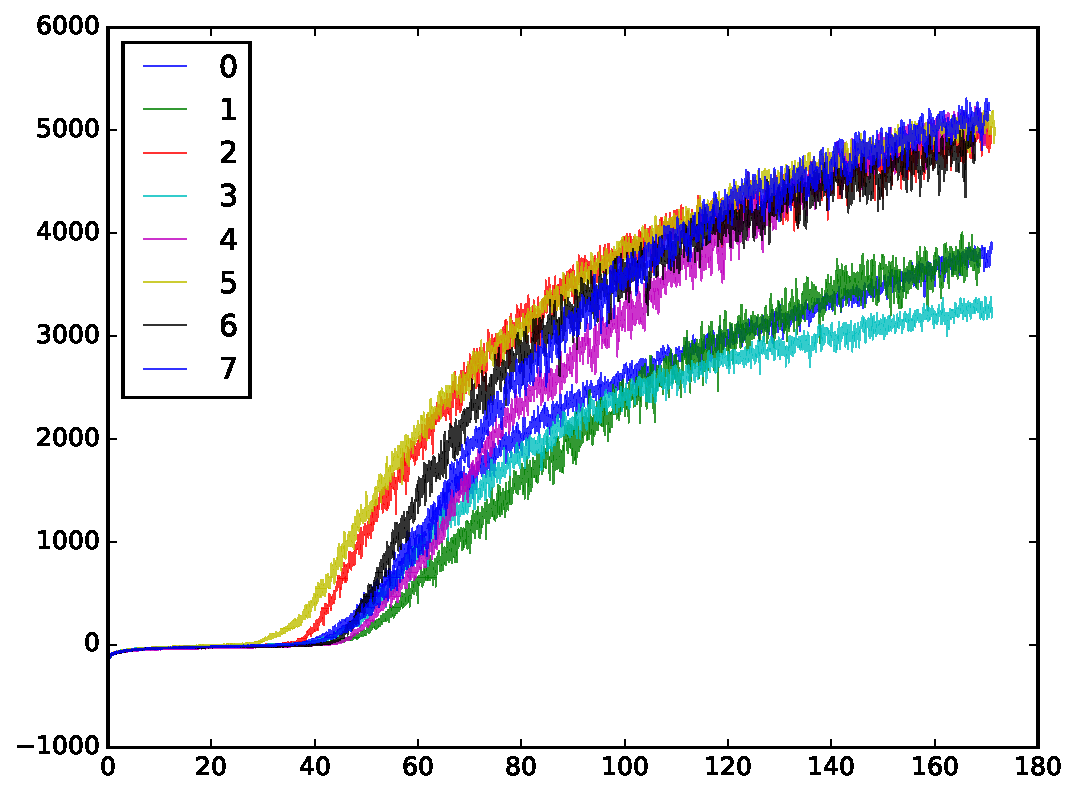
\includegraphics[width=\textwidth]{images/rec_8task_training.pdf}
	\centering
	\caption{Performance of actuator agents with domain randomization by cross-sampling initial states, the x-axis is the number of million time-steps and the y-axis is the total episode reward averaged over the last 200 episodes}\label{rec_8task_training}
\end{figure}

The experiment results of the proposed "synchronous scheduling of actuator learning" is shown in Figure \ref{rec_sync_training}. In this experiments, the agents who outperforms the global lowest-performance by 1000 is paused until it becomes the agent with the lowest performance. The result shows that all the actuator agents reach a final performance of around 6000 although their performance diverge initially.

\begin{figure}[!htbp]
	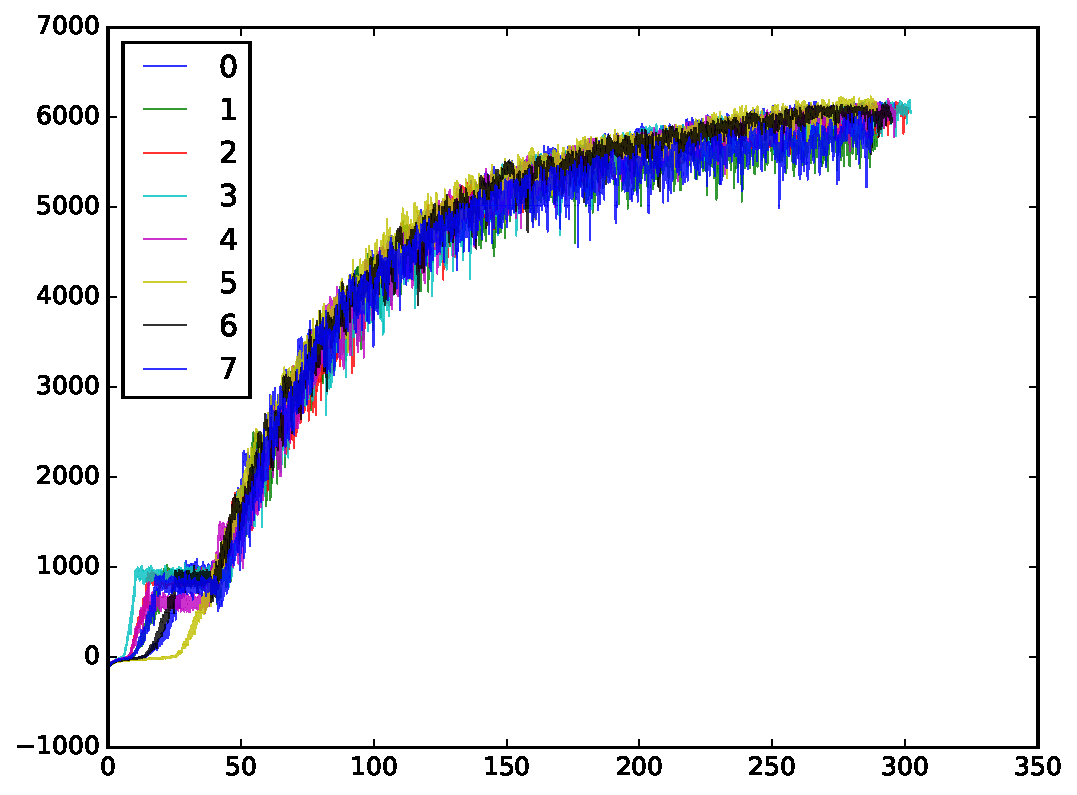
\includegraphics[width=\textwidth]{images/rec_sync_training.pdf}
	\centering
	\caption{Performance of actuator agents using "synchronous scheduling of actuator learning" , the x-axis is the number of million time-steps and the y-axis is the total episode reward averaged over the last 200 episodes}\label{rec_sync_training}
\end{figure}

\subsection{Training of decider agent}
The experiment on the training of decision policy on "dynamicg8" is shown in Figure~\ref{fig:rec_dynamicg8_decider_subt10}. %TODO

\begin{figure}[!htbp]
\centering
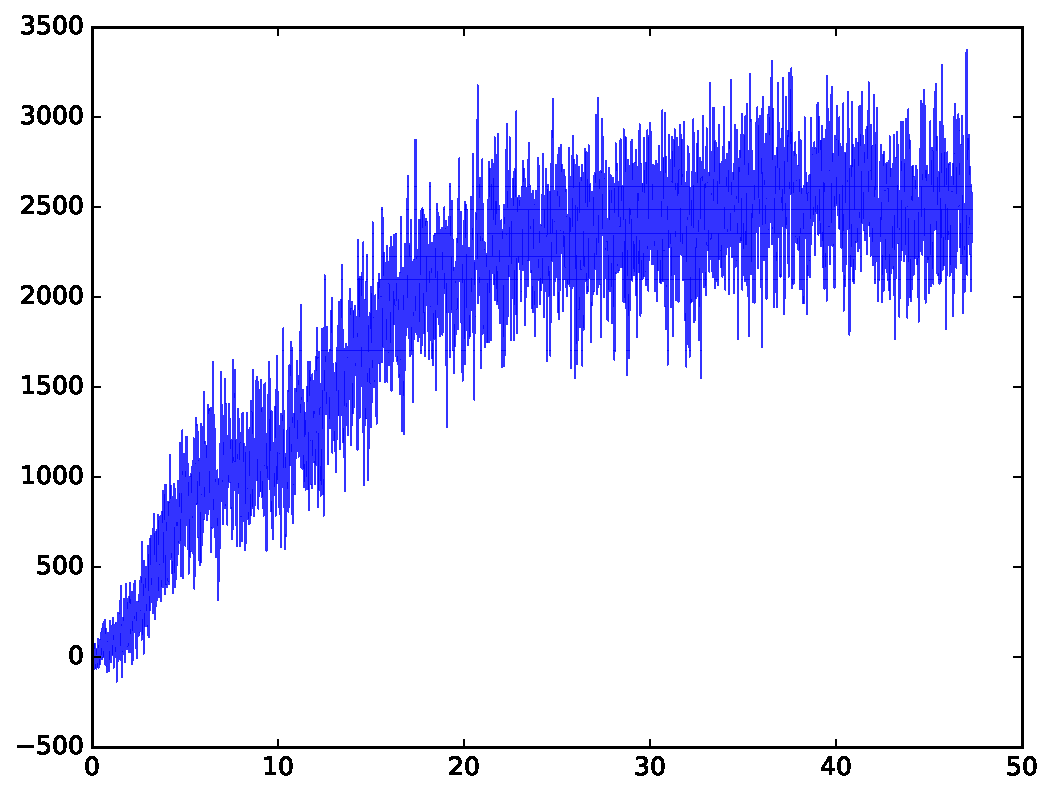
\includegraphics[width=\linewidth]{rec_dynamicg8_decider_subt10}
\caption{Decision policy training performance of the task "dynamicg8", the x-axis is the number of million time-steps and the y-axis is the total episode reward averaged over the last 32 episodes}
\label{fig:rec_dynamicg8_decider_subt10}
\end{figure}

The experiment on the training of decision policy on task "reachcont" is shown in Figure~\ref{fig:rec_reachc05_decider_subt10}.
\begin{figure}
\centering
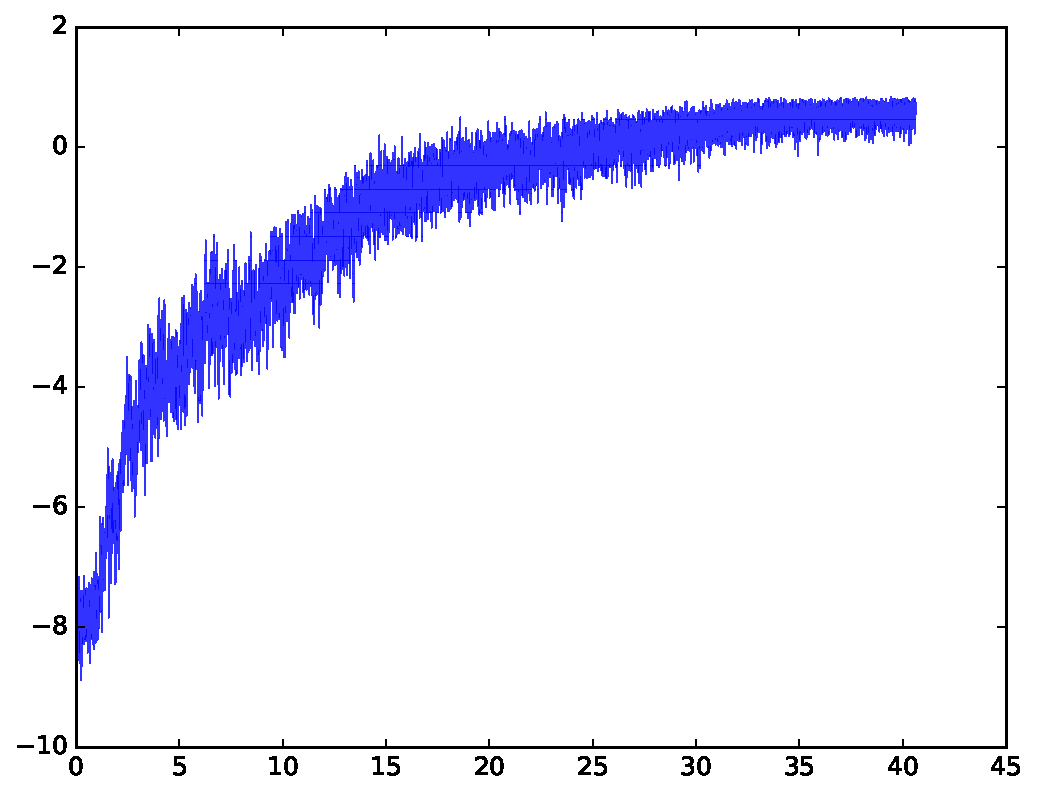
\includegraphics[width=1\linewidth]{rec_reachc05_decider_subt10.pdf}
\caption{}
\label{fig:rec_reachc05_decider_subt10}
\end{figure}


